\section{Introduction}
\subsection{Preface}
\label{cha:Goals}
With the improvement of computers we are able to tackle with high dimensional 
problems in many areas of human life. At first glance everything
looks so easy, but when we go deeper into a problem more and more obstacles
become evident and unavoidable. For example, reconsider pattern recognition
tasks in which measured objects (patterns) coming from the environment can be 
described by many attributes. Some of them are very meaningful while others brings only noise 
and distortion. This is the role of the algorithm to pick valuable attributes,
but finding a minimal attribute reduct is $\mathcal{NP}$-hard problem. Another
important issue is connected with overlaps in the attribute space. When
features are easily separable even a simple classifier works perfectly, but for more 
tricky cases very sophisticated approaches have to be applied.

For the past years, many scientist in the world tried to invent new algorithms
to simplify and improve the accuracy of classification. There are many solutions, 
but ones of the most eminent in the literature are: neural networks, fuzzy logic or 
evolutionary algorithms such as genetic algorithm or tabu search. 
Because simple approaches failed in more complicated problem, scientists tried
to apply algorithms for dimensionality reduction and merge abilities of single
classifier into combined one. This improved the quality of classification 
significantly, but until now no one has managed to invent such a classifier 
that will never make no mistakes.

This thesis touches the broad topic of pattern recognition task which is 
very difficult and demanding problem in every aspect of science. Generally, 
pattern classification is about assigning label to an unknown object based 
on the available knowledge coming from training dataset or expert knowledge.
This process be compared to the capability of human brain which is able to put 
certain scenario into context and identify distinguishable object components. 
The whole process of classification can be divided into into few parts and each 
phase has a significant impact on the final results (more detailed description
about classification task will be presented in section~\ref{cha:Introduction}).

\subsection{Main goals of the  thesis}
Examples of pattern recognition application can be found in many areas of
science. As it was previously noticed, in the literature one can find many algorithms 
used for object classification, while here the rough sets, fuzzy logic and genetic algorithms are used 
and investigated. The general purpose of this thesis is to propose a hybrid
classifier which merges the power of fuzzy logic and rough sets.

First of all the mathematical background and basic properties of these algorithms 
will be presented and later investigations will be carried out to prove 
the usefulness of proposed fusion. It should be noted that for the simulation purposes author
implemented basic fuzzy logic, rough sets algorithms and created a hybrid
classifier.

This thesis is a continuation of work in the field of pattern recognition,
especially connected with rough sets theory. The results of previous experiments can 
be found in \cite{bib34}, \cite{bib35}. 
The aim of this paper is to collect all experiments scenarios in one place and
present the most valuable conclusions for further usage. It is meant to show
the steps of how to construct an advanced hybrid
classifier from the basic algorithms. For this reason, at the beginning of this
thesis the basic properties of rough sets algorithm are checked in simulations, later the algorithm for 
modification decision rules is introduced and at the end as the final point
the hybridization of algorithms is proposed using fuzzy logic, rough sets and
genetic algorithm.

At the end of this section the experiment environment should be characterized in
few words. It is done by defining input/output of the system.
\begin{itemize}
    \item \textbf{given}:
        \begin{itemize}
            \item dataset divided into training and testing objects. in
                this thesis datasets from $UCI$ Repository are used (described in section
                \ref{cha:ExperimentAnalysis}). Those datasets are broadly available and everyone in the
                future would be able to repeat tests and compare the
                results with those presented in this paper,
            \item algorithm for classification: basic rough sets, rough sets
                with modification of decision rules, hybrid classifier,
        \end{itemize}
    \item \textbf{to find}: 
        \begin{itemize}
            \item classification accuracy on the given dataset by the
                particular algorithm,
        \end{itemize}
\end{itemize}
Figure \ref{fig:input_output} shows the general schema of the simulation environment.
\begin{figure}[H]
    \begin{center}
        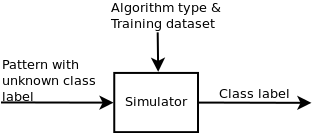
\includegraphics{fig/schema.png}
    \end{center}
    \caption{General schema of simulation environment. Input/output of the
    system}
    \label{fig:input_output}
\end{figure}

\subsection{Scope of this project} 
This paper comprises of two parts. In the first, the review of
literature and the basic notation used in the whole thesis is presented. Section
\ref{cha:Introduction} is the source of the basic
knowledge about pattern recognition. Sections \ref{cha:Rough_set}, \ref{cha:Fuzzy_logic}
present the description of algorithms used in this thesis. Additionally, this
part shows algorithm construction steps using pseudo-code.

The second part, which is the main point of this thesis, presents experiments analysis.
Paragraph \ref{cha:ExperimentAnalysis} describes the experiment environment
settings and program written in \textit{Python} to simulate all implemented
algorithms.  Results with comments are placed in
section \ref{cha:Simulation_investugations}. General
conclusions and plans for the future work are placed in sections
\ref{cha:Summary}, \ref{cha:FutureWork}, respectively. 

